\section{Trigger system firmware development}

After generic trigger system design was complete and hardware components entered production stage firmware development was started. Both HLS and VHDL tools were used. Work was performed using data samples generated by GEMC/GEANT4 package, and cosmic data when hardware components were installed. Present section describes those procedures. Additional development and validation with beam described in \ref{sec:validation}.

\subsection{Simulated data sets preparation}
\label{simulated_data_preparation}

Simulated data sets for trigger system development were prepared using GEMC (GEANT4-based simulation package, \ref). GEMC has realistic CLAS12 geometry and magnetic field map, and produces digitized results suitable to be converted into pre-trigger data format.

Various data sets were generated depending on what was needed for particular trigger component development. For example fixed energy single electron sets were produced for initial EC and PCAL component development. For those sets all detectors before EC or PCAL were disable to make sure single electron is hiting EC or PCAL directly. This way cluster finding algorithm can be developed and tested in ideal conditions. After that realisted data samples were produced and algorithm was tested again.

Another data set was used to create the road dictionary for the Drift Chamber-based trigger component.  For this purpose, positive and negative tracks were generated uniformly  in a selected momentum, $\theta$ and $\phi$ range and tracked through the CLAS12 detector to determine the list of DC wires involved by the particle trajectory. More details can be found in Section \ref{dc_dictionary}.


\subsection{Development using simulated data}

Development process consists of several methods and depends on the nature of the trigger component. Most stage1 components were implemented using HLS/VIVADO tool, where firmware was written using HLS C++ extension. In that case it was possible to develop and validate firmware as part of offline reconstruction framework using regilar desktop. Usually the offline processing alghorithms were re-written using HLS/C++, with appropriate simplification and structural changes to make it sutable for FPGA firmware. Simulated data were used as input, they were processed directly by HLS/C++ code and compared with initial similation parameters. In addition, the same samples were processed by offline reconstruction software and results compared with the trigger output. That double check method practicaly guarantees bug-free implementation. It was no single case when C++ implementation passed tests on simulated data and failed on final validation stage. Most complicated stage1 components were developed and tested using this method.

Several components of the trigger were written mostly in VHDL and initially no software existed for feeding GEMC data into HDL simulations. This was the case for stage 1 FT and DC tracking trigger as well as stage 2 and stage 3 components of the trigger. These modules relied on standard VHDL test benches to feed/generate test vectors for evaluating the correctness of the design modules. For example, the FT testbench generated clusters at each position of the calorimeter and hodoscope to test channel mapping and geometry matching. Additional specific test cases verified the FT trigger clustering time coincidence, cluster multiplicity, and latency to ensure it operated as expected. C/C++ modules were written which emulated the FT the DC tracking trigger so the algorithms could work in the same offline framework as described above for other stage 1 components.

\subsection{Development and validation using cosmic data}

When hardware components for CLAS12 detector were produced and mostly installed, and first version of firmware was ready for testing, all three trigger system stages firmwares were loaded and development continues for entire trigger system using cosmic data. At that point we started to perform trigger system validation for some components, while development was continue for others, as described in following sections.

\subsubsection{Alternative 'hit-based' trigger system}

CLAS12 detector inheritated some components from previously existed CLAS detector, in particular its trigger system. That system was feeded by tdc/discriminator boards and was able to produce 'hit-based' information only. We desided to keep it for reference purposes as alternative for the new trigger system. It was used during cosmic data CLAS12 detector calibration and new trigger system validation up to the point when new trigger system was ready. It is still operational and can be used to double-check of the main CLAS12 trigger system if needed.

\subsubsection{Development and validation of EC/PCAL special purpose trigger with cosmic data}

First step in cosmic data usage was detectors calibration. It was performed for all CLAS12 detectors and described in corresponding articles. Here we will describe, as an example, one of the procedures related to EC/PCAL calibration needed for correct trigger system performance. Similar procedures were executed for all detectors participating in trigger system.

Efficiency and spatial uniformity of cluster finding trigger in EC/PCAL described in Section 5.3 requires already calibrated calorimeters with pre-determined PMT gain and light attenuation constants loaded into the VTP/FPGA trigger firmware.  Calibration runs using a special purpose MIP trigger were used to obtain these constants. For that purpose so-called "pixel trigger" was developed and loaded into stage1 firmware along with main trigger, so it was possible to calibrate the system using pixel trigger and then switch to the main one for data taking. This "pixel trigger" used a simple multiplicity condition on 1D cluster size for each U,V,W view to reject undesirable muon trajectories and select normally incident tracks.  This reduced the trigger and data rate by 95$\%$ and ensured the same MIP energy was deposited for all possible triple intersections of single strips.

The pixel trigger pipeline executes these steps in parallel, with user configurable parameters in bold:
  1) If FADC hit energy $>$ \textbf{EMIN}, make a pulse \textbf{HITWIDTH}*4ns for that strip.
  2) Look for coincidence of U,V,W pixel strip candidates from step 1.
  3) Evaluate multiplicity \textbf{EVALDELAY}*4ns clock cycles after the leading edge of a candidate pixel from step 2.
  4) Generate pixel trigger if multiplicity requirement is met and we still have a hit on U,V,and W. 

Additional configurable trigger elements were introduced, including a total energy sum threshold \textbf{ESUM} and a lookup table for triplets of strips which satisfy the geometrical constraint $dU+dV+dW=\textbf{DALITZ}$, where $d$ is the normalized distance to the hit strip indicated by the arrows in Fig. 6 and $\textbf{DALITZ}=2$ for perfect pixels.  The latter test was sometimes necessary to prevent noisy PMTs from saturating the multiplicity (N=3) trigger condition.  Offline analysis showed that about $90\%$ of pixel triggers satisfied the Dalitz test (Fig. 7), while adjacent calorimeter elements which did not use the trigger had a much smaller pixel fraction.  This suggests the pixel trigger helps to suppress events which undergo multiple scattering, which would trigger adjacent strips and violate the multiplicity requirement.
%%%%%%%%%%%%%%%%%%%%%%%%%%%%%%%%%%%%%%%%% F I G U R E %%%%%%%%%%%%%%%%%%%%%%%%%%%%%%%%%%%%%%%%%%
\begin{figure}[!htb]
 \centering
  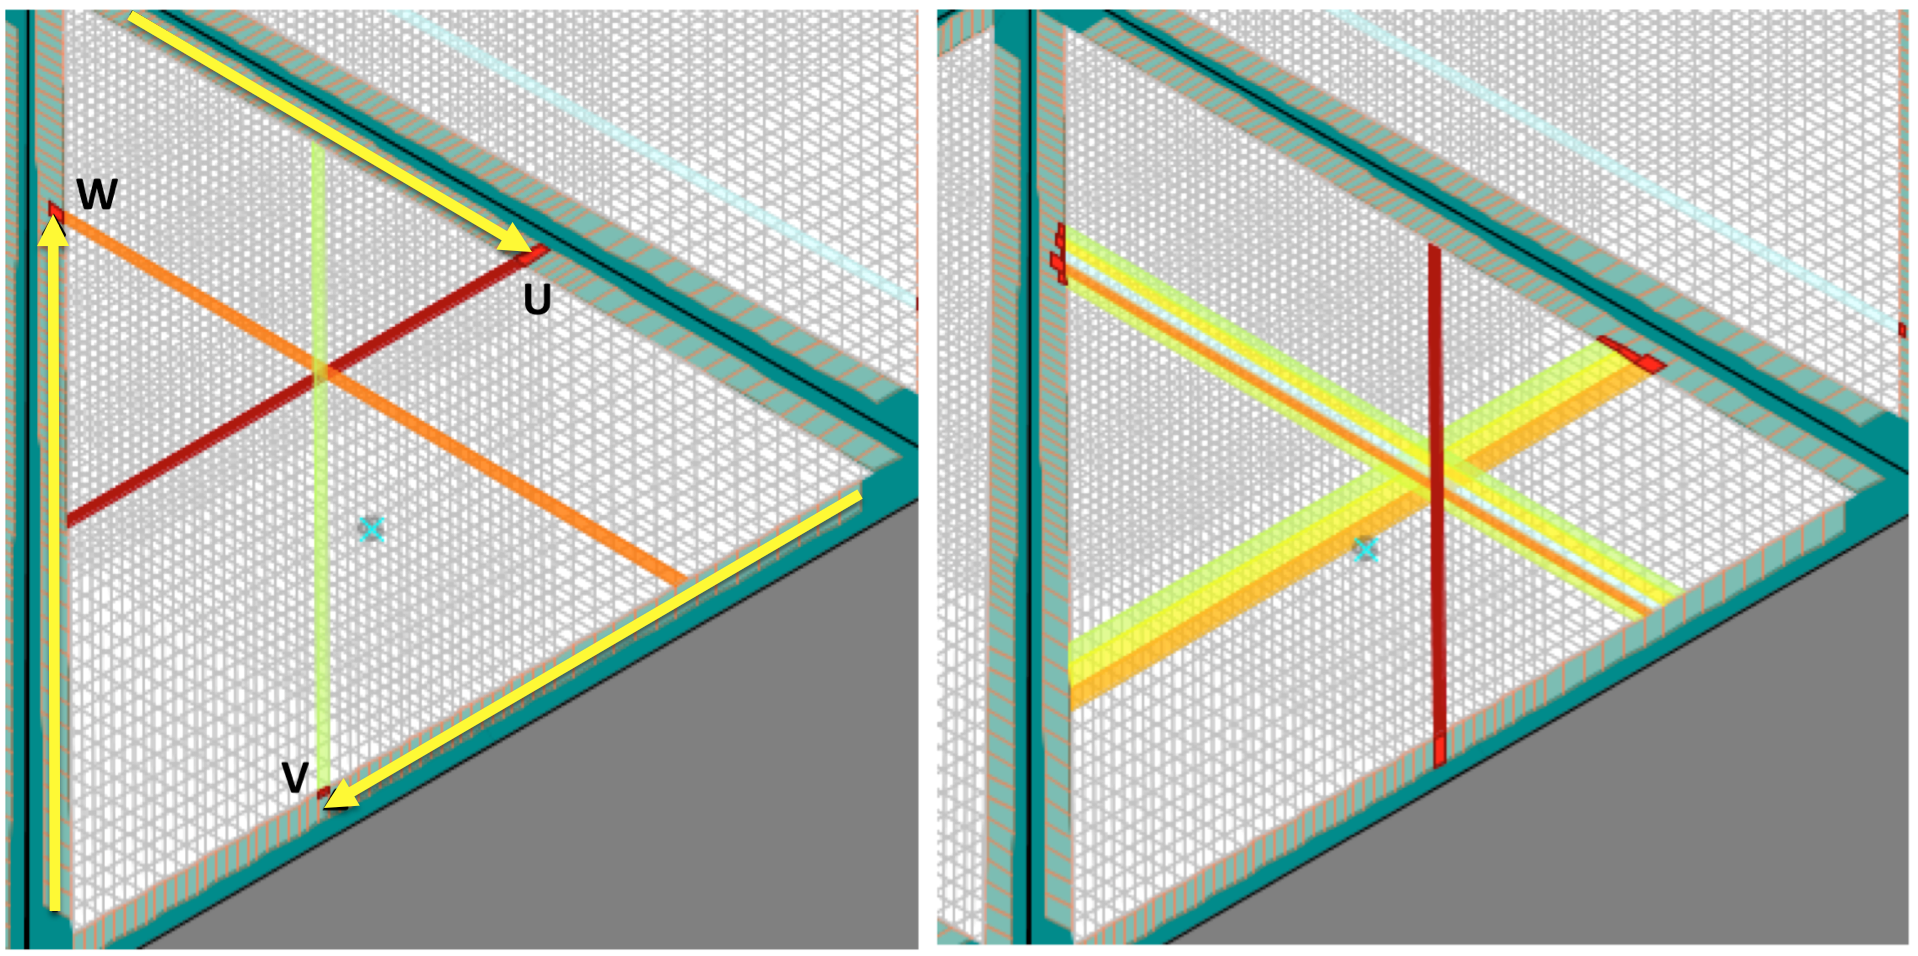
\includegraphics[width=0.95\columnwidth,keepaspectratio]{img/TwoClusters.png}
 \caption{Examples of clusters from cosmic muon triggers.  Desired trajectory (left) is normally incident on the face of PCAL and satisfies the single pixel multiplicity condition (N$_u$=N$_v$=N$_w$=1) in the FPGA pixel trigger.  Event at right shows a more vertical trajectory rejected by this trigger.}
\end{figure}
%%%%%%%%%%%%%%%%%%%%%%%%%%%%%%%%%%%%%%%%% F I G U R E %%%%%%%%%%%%%%%%%%%%%%%%%%%%%%%%%%%%%%%%%%

%%%%%%%%%%%%%%%%%%%%%%%%%%%%%%%%%%%%%%%%% F I G U R E %%%%%%%%%%%%%%%%%%%%%%%%%%%%%%%%%%%%%%%%%%
\begin{figure}[!htb]
 \centering
  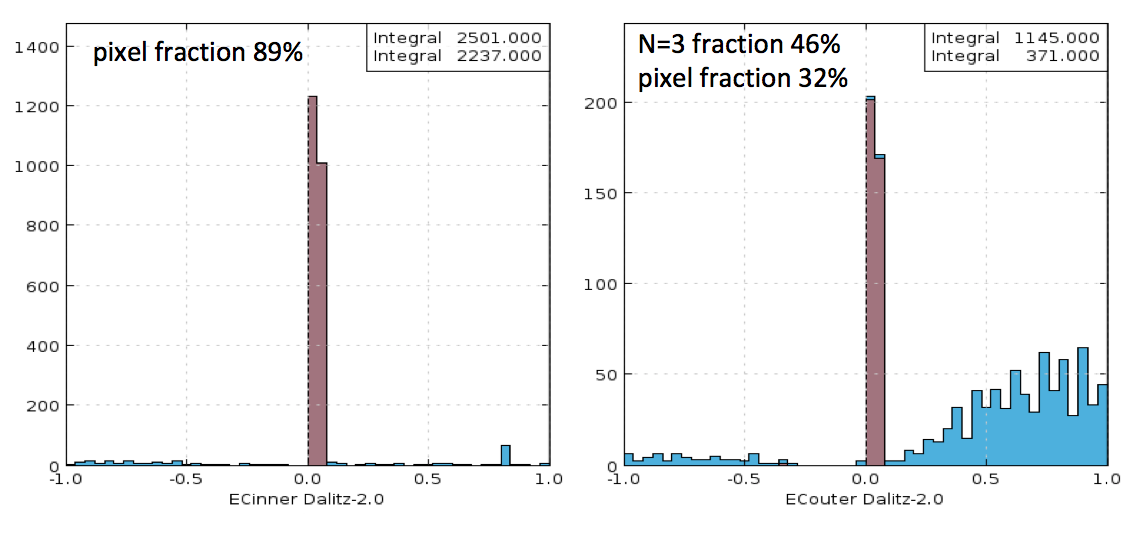
\includegraphics[width=1.0\columnwidth,keepaspectratio]{img/PixelFraction.png}
 \caption{Offline analysis of events which satisfied the pixel trigger on ECINNER calorimeter.  Left plot shows 89$\%$ of ECINNER triggers satisfied the pixel test $dU+dV+dW=2$.  Right plot shows only 14$\%$ of the ECINNER triggers found an ECOUTER event that satisfied both the $N=3$ and pixel test. }
\end{figure}
%%%%%%%%%%%%%%%%%%%%%%%%%%%%%%%%%%%%%%%%% F I G U R E %%%%%%%%%%%%%%%%%%%%%%%%%%%%%%%%%%%%%%%%%%

\subsubsection{Development and validation of entire trigger system with cosmic data} 

While stage1 trigger components were validated separately from each other on development stage, stage2 and stage3 components requires entire system to be assembled to perform validation. Initially those two stages were programmed with simplified alghorithms to test signals propagation and basic trigger system functionality, only timing coincidense between different detectors was implemented. Development of stage2 and stage3 continues during cosmic run operations and later with beam operations, adding geometrical match between different detectors and increasing coincidense logic complexity.

\subsubsection{Development and validation of drift chamber component of the trigger system with beam data}



\subsubsection{Trigger system flexibility and 'permanent development' mode}

Initial plan was to develop trigger system firmware which will satisfy all CLAS12 experiments for entire course of CLAS12 operation, meaning high (close to 100\%) trigger efficiency and reasonable purity. As the power and flexibility of the trigger system was revealed to community, additional requirements were placed to improve system purity, and to include additional physics processes. As result stage2 and stage3 components of the trigger system were under constant development during first year of CLAS12 operation, firmware was upgraded and entire system validated after every change. After a while trigger system reached the point when relatively small improvement in trigger purity can be achieved with significant efforts, after that development was declared complete. The nature of the fpga-based trigger system allows almost endless improvements, but such 'permanent development' mode seems not practical.
